\documentclass[10pt]{article}
\usepackage{tikz}
\pagestyle{empty}

\begin{document}

\vspace*{\fill}
\begin{center}
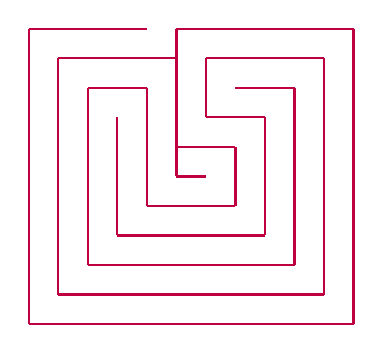
\begin{tikzpicture}[scale = 1.5, x = 0.25cm, y = -0.25cm, thick, purple]
% Horizontal lines
\draw(0, 0) -- (4, 0);
\draw(0, 10) -- (11, 10);
\draw(1, 1) -- (5, 1);
\draw(1, 9) -- (10, 9);
\draw(2, 2) -- (4, 2);
\draw(2, 8) -- (9, 8);
\draw(3, 7) -- (8, 7);
\draw(4, 6) -- (7, 6);
\draw(5, 0) -- (11, 0);
\draw(5, 4) -- (7, 4);
\draw(5, 5) -- (6, 5);
\draw(6, 1) -- (10, 1);
\draw(6, 3) -- (8, 3);
\draw(7, 2) -- (9, 2);
% Vertical lines
\draw(0, 0) -- (0, 10);
\draw(1, 1) -- (1, 9);
\draw(2, 2) -- (2, 8);
\draw(3, 3) -- (3, 7);
\draw(4, 2) -- (4, 6);
\draw(5, 0) -- (5, 5);
\draw(6, 1) -- (6, 3);
\draw(7, 4) -- (7, 6);
\draw(8, 3) -- (8, 7);
\draw(9, 2) -- (9, 8);
\draw(10, 1) -- (10, 9);
\draw(11, 0) -- (11, 10);
\end{tikzpicture}
\end{center}
\vspace*{\fill}

\end{document}
